
%(BEGIN_QUESTION)
% Copyright 2014, Tony R. Kuphaldt, released under the Creative Commons Attribution License (v 1.0)
% This means you may do almost anything with this work of mine, so long as you give me proper credit

Denne gruppen stolpemonterte krafttransformatorer transformerer 7.2 kVAC linjespenning ned til 120/208 VAC for å forsyne en liten bedrift:

$$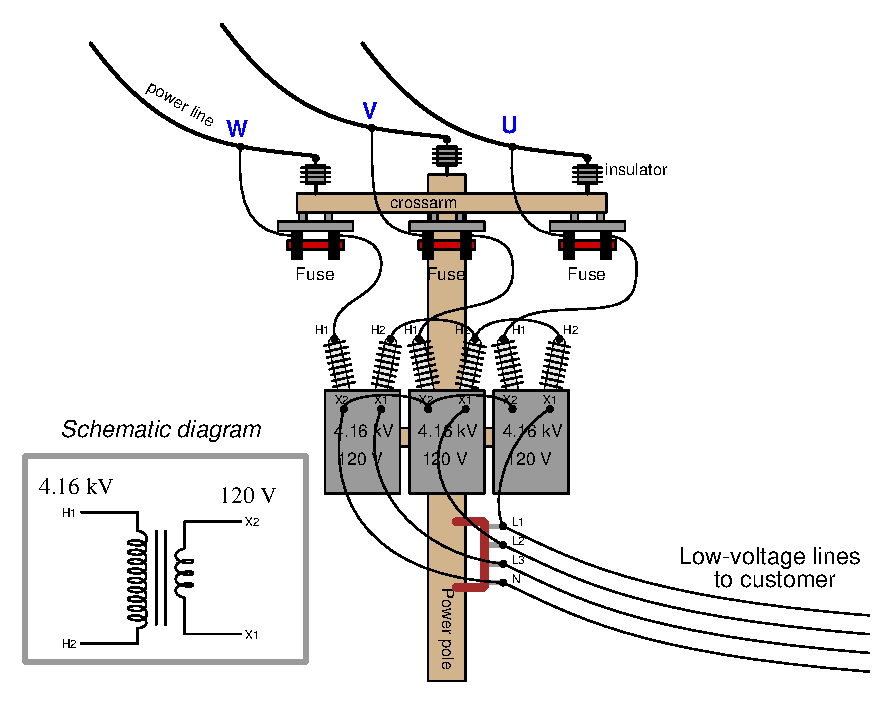
\includegraphics[width=15.5cm]{i00821x01.eps}$$

Gitt følgende linjespenninger (målt fase-mot-jord), beregn fasevinklene for de oppgitte sekundærspenningene:

\begin{itemize}
\item{} $V_U$ = 4160 V $\angle$ $0^o$
\item{} $V_V$ = 4160 V $\angle$ $-120^o$
\item{} $V_W$ = 4160 V $\angle$ $-240^o$
\end{itemize}

\vskip 10pt

\begin{itemize}
\item{} $V_{L1-N}$ = \underbar{\hskip 20pt} $\angle$ \underbar{\hskip 10pt}
\vskip 5pt
\item{} $V_{L2-N}$ = \underbar{\hskip 20pt} $\angle$ \underbar{\hskip 10pt}
\vskip 5pt
\item{} $V_{L3-N}$ = \underbar{\hskip 20pt} $\angle$ \underbar{\hskip 10pt}
\vskip 5pt
\item{} $V_{L1-L3}$ = \underbar{\hskip 20pt} $\angle$ \underbar{\hskip 10pt}
\end{itemize}

\vskip 20pt \vbox{\hrule \hbox{\strut \vrule{} {\bf Forslag til sokratisk diskusjon} \vrule} \hrule}

\begin{itemize}
\item{} Har disse krafttransformatorene {\it additiv} eller {\it subtraktiv} polaritet? Hvordan ser du det?
\item{} Identifiser fasesekvensen (fase{\it rotasjon}) i dette kraftsystemet basert på oppgitte fase-mot-jord-verdier.
\end{itemize}

\underbar{file i00821}
%(END_QUESTION)





%(BEGIN_ANSWER)

\noindent
{\bf Delsvar:}

$$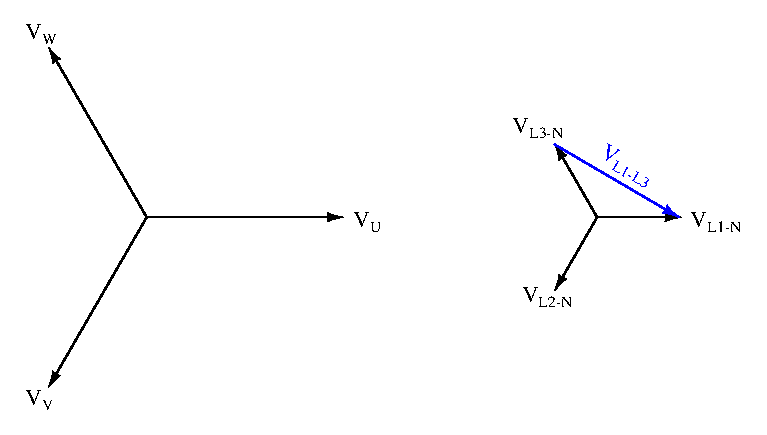
\includegraphics[width=15.5cm]{i00821x02.eps}$$

%(END_ANSWER)





%(BEGIN_NOTES)

Når hver transformator får 4160 volt på primærviklingen, vil hver sekundærvikling gi 120 volt med samme fasevinkel som tilsvarende primærfase. Dermed:

\begin{itemize}
\item{} $V_{L1-N}$ = 120 V $\angle$ $0^o$
\vskip 5pt
\item{} $V_{L2-N}$ = 120 V $\angle$ $-120^o$
\vskip 5pt
\item{} $V_{L3-N}$ = 120 V $\angle$ $-240^o$
\end{itemize}

Linjespenningen $V_{L1-L3}$ kan beregnes symbolsk ved å trekke $V_{L3-N}$ fra $V_{L1-N}$:

$$V_{L1-L3} = V_{L1-N} - V_{L3-N}$$

$$V_{L1-L3} = (120 \hbox{ V} \angle 0^o) - (120 \hbox{ V} \angle -240^o)$$

$$V_{L1-L3} = 207.85 \hbox{ V} \angle -30^o$$

Samme spenning kan også beregnes grafisk ved å tegne fasoren $V_{L1-L3}$ mellom spissene til fasorene $V_{L1-N}$ og $V_{L3-N}$:

$$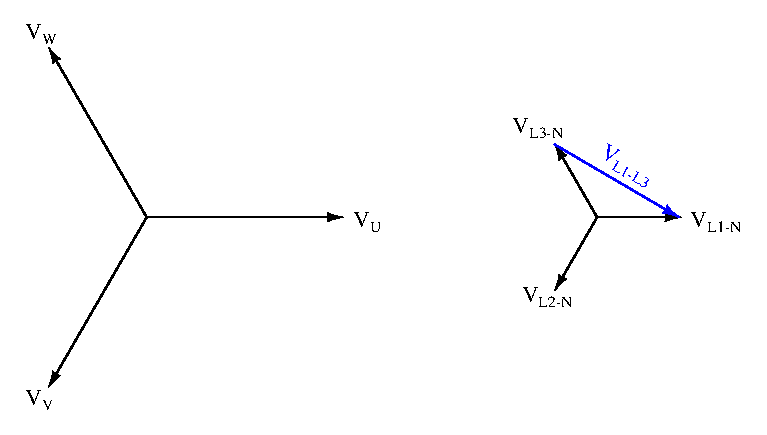
\includegraphics[width=15.5cm]{i00821x02.eps}$$

%INDEX% Electronics review: AC transformer circuit
%INDEX% Electronics review, phasor expressions of circuit quantities
%INDEX% Electronics review, 3-phase transformer bank phase shift calculations

%(END_NOTES)
